\documentclass[UTF8]{ctexart}

\usepackage{subfiles}  

%下面的语句, 引入你的头部设置文件
\usepackage{C:/phpStorm_proj/02_myself_ID_EGO/+100_latex_all_math_sel/myPreamble} 
%必须是绝对路径,才能让各个tex在单独编译时使用到

\title{文件名}


%---------------------------------


\begin{document}
	\tableofcontents % 生成目录
	\date{} % 若不写这句, 则默认也会渲染出日期, 所以我们要手动赋空值
	\maketitle  %这行代码, 让你前面的 title, author, date生效
	
	


	
	\part{指数分布 Exponential distribution}
	
	\section{指数分布 : 若一段时间内, 随机事件\underline{发生的次数, 呈``泊松分布"}. 那么,这些随机事件\underline{发生的时间间隔, 便呈``指数分布"}.}
	
	\textbf{``指数分布"与``泊松分布"密切相关:如果在某时间段内, 随机事件发生的次数, 呈``泊松分布". 那么,这些随机事件之间的时间间隔, 便呈``指数分布".} \\
	
	\begin{myEnvSample}
	回想一下: ``泊松分布" 是描述单位时间内, 随机事件发生的次数. \\

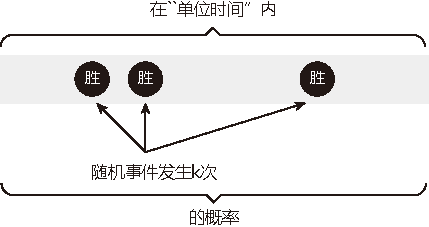
\includegraphics[width=0.55\textwidth]{/0156.pdf} \\

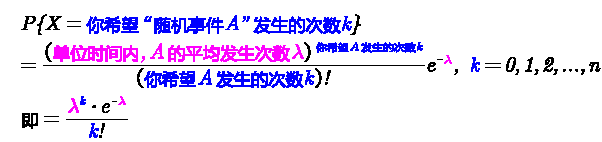
\includegraphics[width=0.8\textwidth]{/0149.pdf} \\
所以, 泊松分布的``概率函数"就是: $\boxed{
	P\left(X=\text{你想要发生的次数} \right) =\frac{\text{均}^{\text{想}}\cdot e^{-\text{均}}}{\text{想!}}
}$
	\end{myEnvSample}

	
	例如, 如果抵达某家银行的客户人数呈``泊松分布",比如说 $\lambda$=12人/小时 ($\lambda$, 是单位时间(或单位面积)内, 随机事件的\textbf{平均发生次数}). 那么,他们抵达的时间间隔, 则呈``指数分布",平均值 $\mu$=1/12,或者说5分钟. \\
	
	\begin{tabular}{|l|l|}
		\hline
		``泊松分布"中的参数$\lambda$ : &  是单位时间(或单位面积)内, 随机事件的\textbf{平均发生次数}.\\
		\hline
			``指数分布"中的参数 $\mu$ : &  表示``随机事件发生的\textbf{平均时间间隔}". 它与 $\lambda$ 的关系是 : $ \boxed{ \lambda = \dfrac{1} {\mu}}$.\\
		\hline
	\end{tabular} \\

即,``指数分布"可以用来表示: 独立随机事件\textbf{发生的时间间隔}. 比如 : \\
- 旅客进入机场的时间间隔. \\
- 电话打进客服中心的时间间隔. \\
- twitter上用户发表新微博的时间间隔. \\
- 机器的寿命等 (许多电子产品的寿命分布, 一般服从"指数分布"). \\









\section{指数分布的``概率函数": $\boxed{f\left( x;\lambda \right) =\lambda \cdot e^{-\lambda x}\ (x>0)		}$}


若一个随机变量X呈``指数分布", 则可以写作:$\boxed{X \sim E(\lambda)}$. \\

  
指数分布的``概率函数"是: \\
$\boxed{
f\left( x;\underset{\text{每单位时间内,随机事件发生的次数}}{\underbrace{\lambda }} \right) =\left\{ \begin{array}{l}
	\lambda \cdot e^{-\lambda x}\ (x>0)\\
	0\ (x\leq 0)\\
\end{array} \right. 
}$ \\
其中, $\lambda$ 表示: 每``单位时间"内, 随机事件的发生次数. 

或: \\
$ \boxed{
f\left( x;\underset{\text{随机事件,在每单位时间内的发生率}}{\underbrace{\beta }} \right) =\left\{ \begin{array}{l}
	\dfrac{1}{\beta}\cdot e^{-\frac{1}{\beta}x}\ (x\ge 0)\\
	0\ (x<0)\\
\end{array} \right. 
}$  \\
其中, $\beta$ 表示: 随机事件, 在``每单位时间"内的``发生率".\\
 
 
``概率函数"图如下: \\
 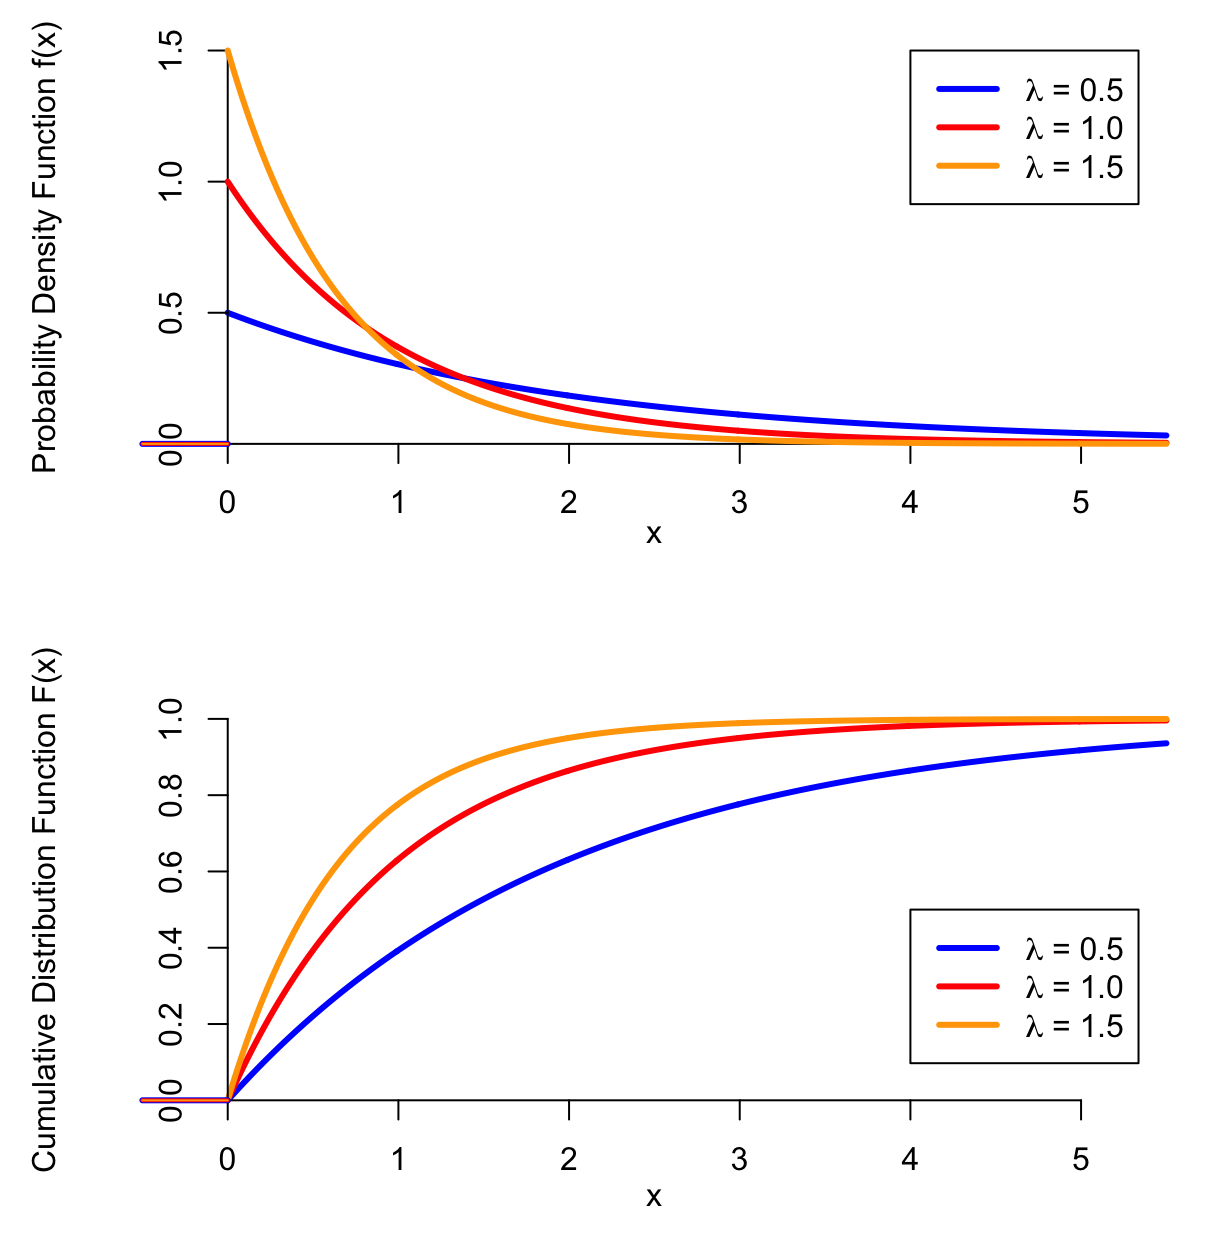
\includegraphics[width=0.6\textwidth]{/0179.png} \\

从图上可以看出: \\
- 指数分布的x区间是[0,∞). \\
- 指数分布, 它的y值是有下限的, =0. \\
- 在x=0处, 函数有最大的y值. \\
- 函数为右偏. 且随着x的增大, 函数的y值稳步下降 (即是个减函数). \\
- 其中的参数 $\lambda >0$, 它表示``每单位时间内, 发生某事件的次数". 它常被称为``率参数" (rate parameter). \\

 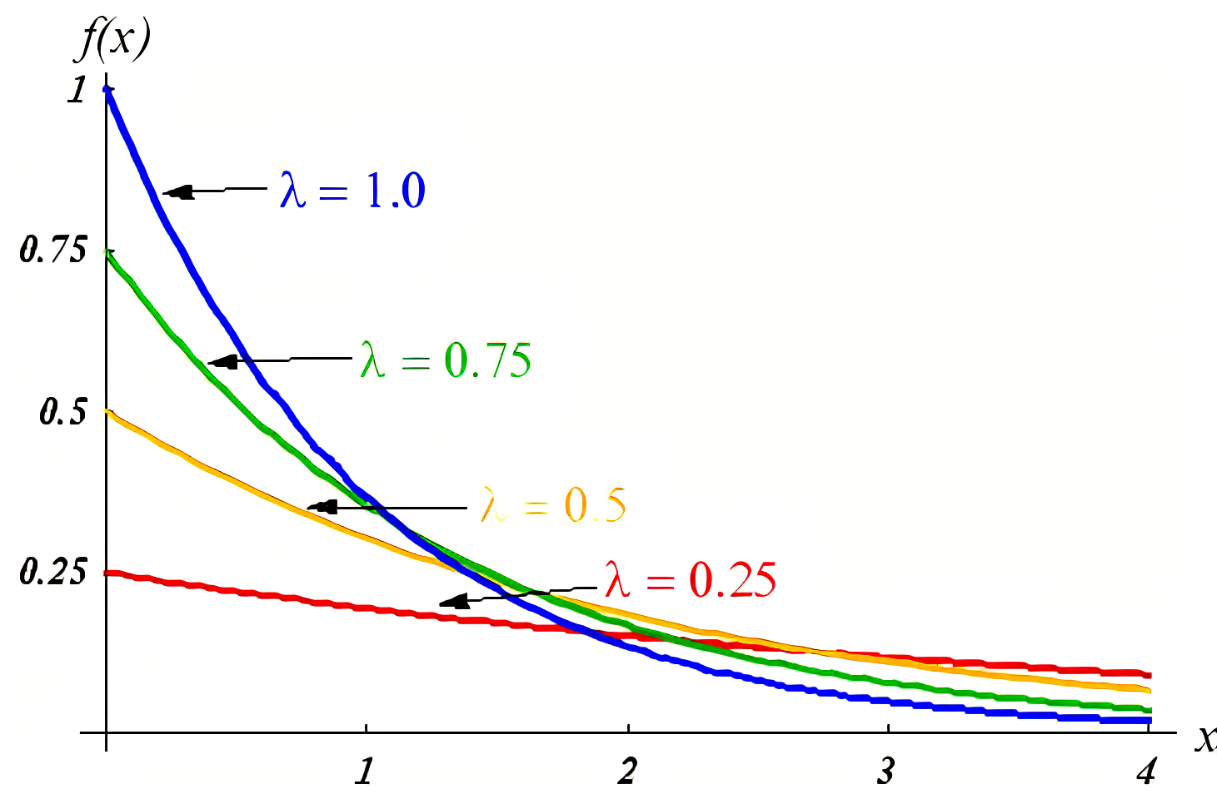
\includegraphics[width=0.5\textwidth]{/0178.png} \\


这个``指数分布 Exponential distribution"的``概率函数"图形, 表面上看与``幂律分布 Power law distribution"很相似, 其实两者有极大不同 : \textbf{``指数分布"的收敛速度, 要远快过``幂律分布".} \\







\section{指数分布的``累加函数": $\boxed {F(x)=1-e^{-\lambda x}\ (x>0)}$}

$\boxed{
F(x) = \begin{cases}
	1- e^{-λx} & \quad x>0 \\
	0 &  \quad x \leq 0  \\
\end{cases} }$ \\
\vspace{1em} 


\begin{myEnvSample}
一台发动机的某个关键零件, 出故障的``平均间隔时间" μ=8000小时. 则, 单位时间(1小时)内, 出故障的次数就是 :
\begin{align*}  % 支持每行编号. 若不需要编号, 就用 align*环境
	&\frac{\text{出1次故障}}{8000\text{小时}}\ \gets \text{分子分母同时除以}8000\\
&=\frac{\frac{\text{出1次故障}}{8000}}{1\text{小时}}\ \gets \text{即每1小时}(\text{单位时间}),\ \text{出}\frac{1}{8000}\text{次故障}
\end{align*}

因为该随机事件(机器出故障), 可用``指数分布"来模拟. 所以, 如果我们要求``它在5000小时之前会出故障"的概率, 就用``累加函数"来算了. \\

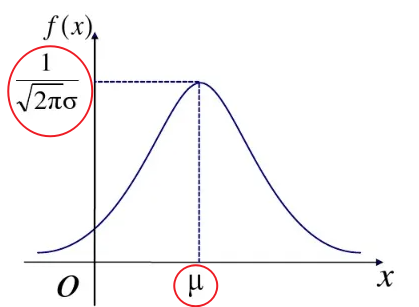
\includegraphics[width=0.55\textwidth]{/0180.png} \\

mathematica 中的计算 : \\
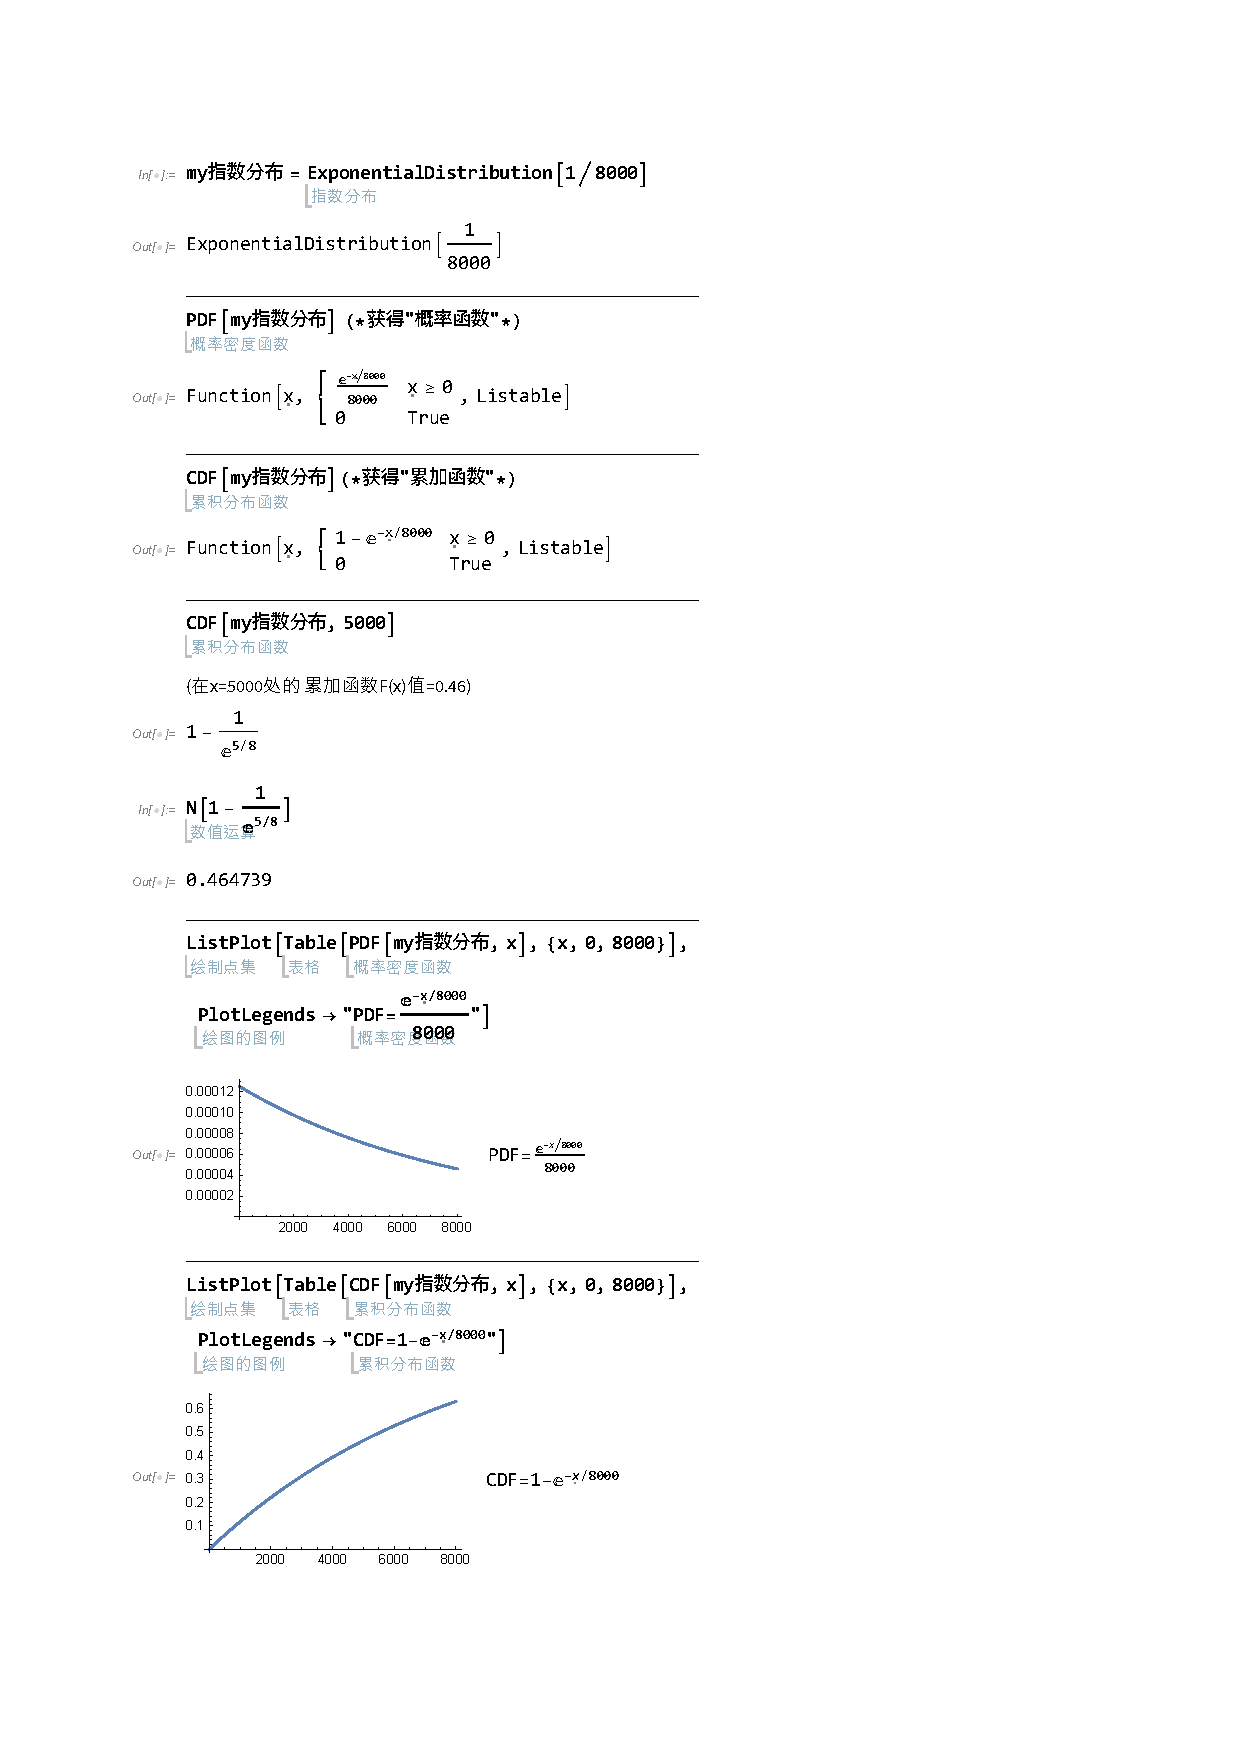
\includegraphics[width=0.7\textwidth]{/0181.pdf} 
\end{myEnvSample}
\vspace{1em} 



\begin{myEnvSample}
	有一堆元件, 寿命用X表示, 服从``指数分布". \\
	其概率函数是: $
	f\left( x \right) =\left\{ \begin{array}{l}
		\lambda \cdot e^{-\lambda x}=\frac{1}{1000}e^{-\frac{1}{1000}x}\ \left( x>0 \right)\\
		0\ \left( x\leq 0 \right)\\
	\end{array} \right. 
	$ \\
	
	某机器上, 含有3个这种元件. 其中只要坏掉1个元件, 整个机器就坏掉. \\
	问 : 该机器能工作到1000小时以上的概率? \\
	
	其实就是求: ``这3个元件, 能同时保持正常状态到1000小时以上"的概率. \\
	
	→ 我们先求1个元件, 能``保持正常状态, 超过1000小时"的概率 : \\
	$
	P\left\{ X>1000 \right\} =\int_{1000}^{+\infty}{\left[ \underset{\text{即概率函数}f(x)}{\underbrace{\frac{1}{1000}e^{-\frac{1}{1000}x}}} \right]}dx=-e^{-\frac{1}{1000}x}\mid_{1000}^{+\infty}=e^{-1}=0.367879
	$ \\
	
	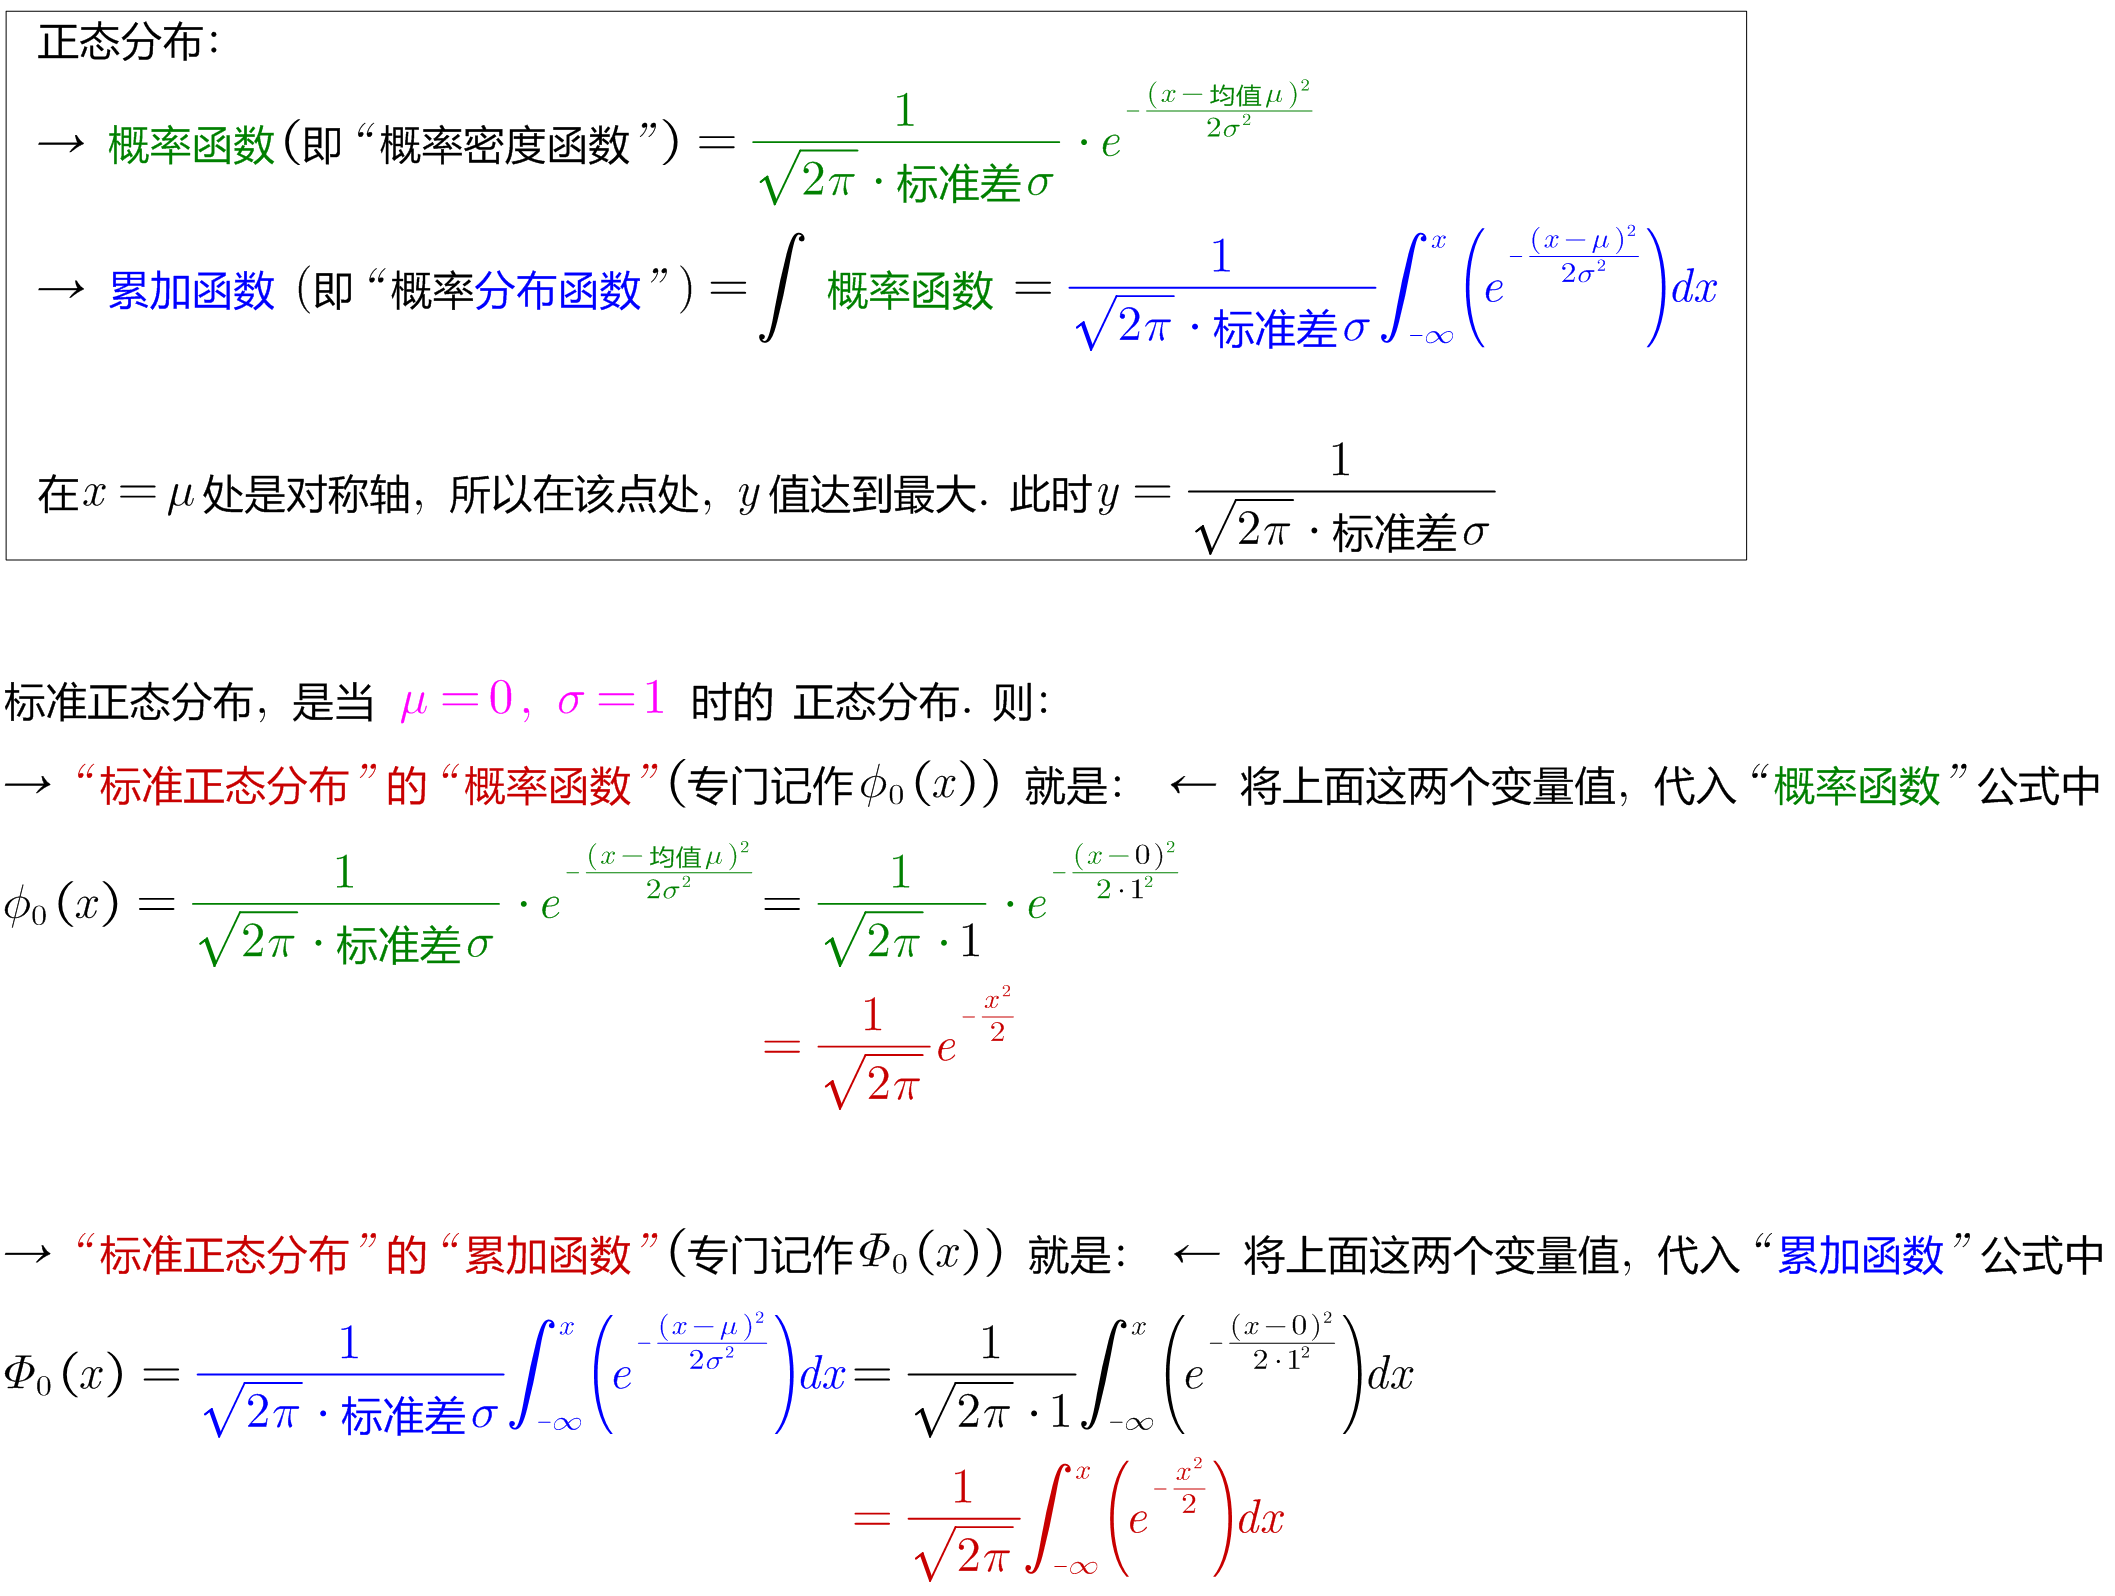
\includegraphics[width=0.55\textwidth]{/0182.png} \\
	
	→ 所以, 同时有3个都能满足``保持正常状态, 超过1000小时"的概率就是 : \\
	$
	\left[ P\left\{ X>1000 \right\} \right] ^3=(e^{-1})^3=e^{-3}=0.0497871
	$ \\
	
	
	
\end{myEnvSample}






\section{指数分布, 具有``无记忆" }

但是,由于指数分布具有缺乏“记忆”的特性, 因而限制了它在``机械可靠性"研究中的应用. \\

\textbf{所谓缺乏``记忆”,是指它假设: 某种产品或零件, 经过一段时间t0 的工作后, 仍然如同全新的产品一样,不影响以后的工作寿命值 (换言之, 它忽略了``磨损或风蚀"会对产品寿命有``缩短"的影响).} \\
即, ``无记忆性"就是说:  一个灯泡, 你用了n年后, 它能再用1年的概率, 和它刚买时, 能再用1年的的概率, 是相等的.  即, 在``指数分布"里, 一个东西的寿命, 对``已使用时间"是没有记忆的. \\

\textbf{或者说, 它假设: 经过一段时间t0 的工作之后, 该产品的寿命分布, 与原来还未工作时的寿命分布相同.} \\

所以, ``指数分布"只能近似地来作为机器或系统的``失效分布模型". \\
	
	
无记忆性, 就是说:	\\
$ \boxed{
P\{X>s+t\ |\ \text{当}X>s\text{时\}}=P\{X>t\},\ \ for\ a,x>0
}$ \\

这个等式也就是说 : ``X 超过 s+t" 的概率, 和 ``超过t"的概率, 是相等的. 换言之, 这个概率``无视t的存在与否", 都不影响概率本身的值. \\

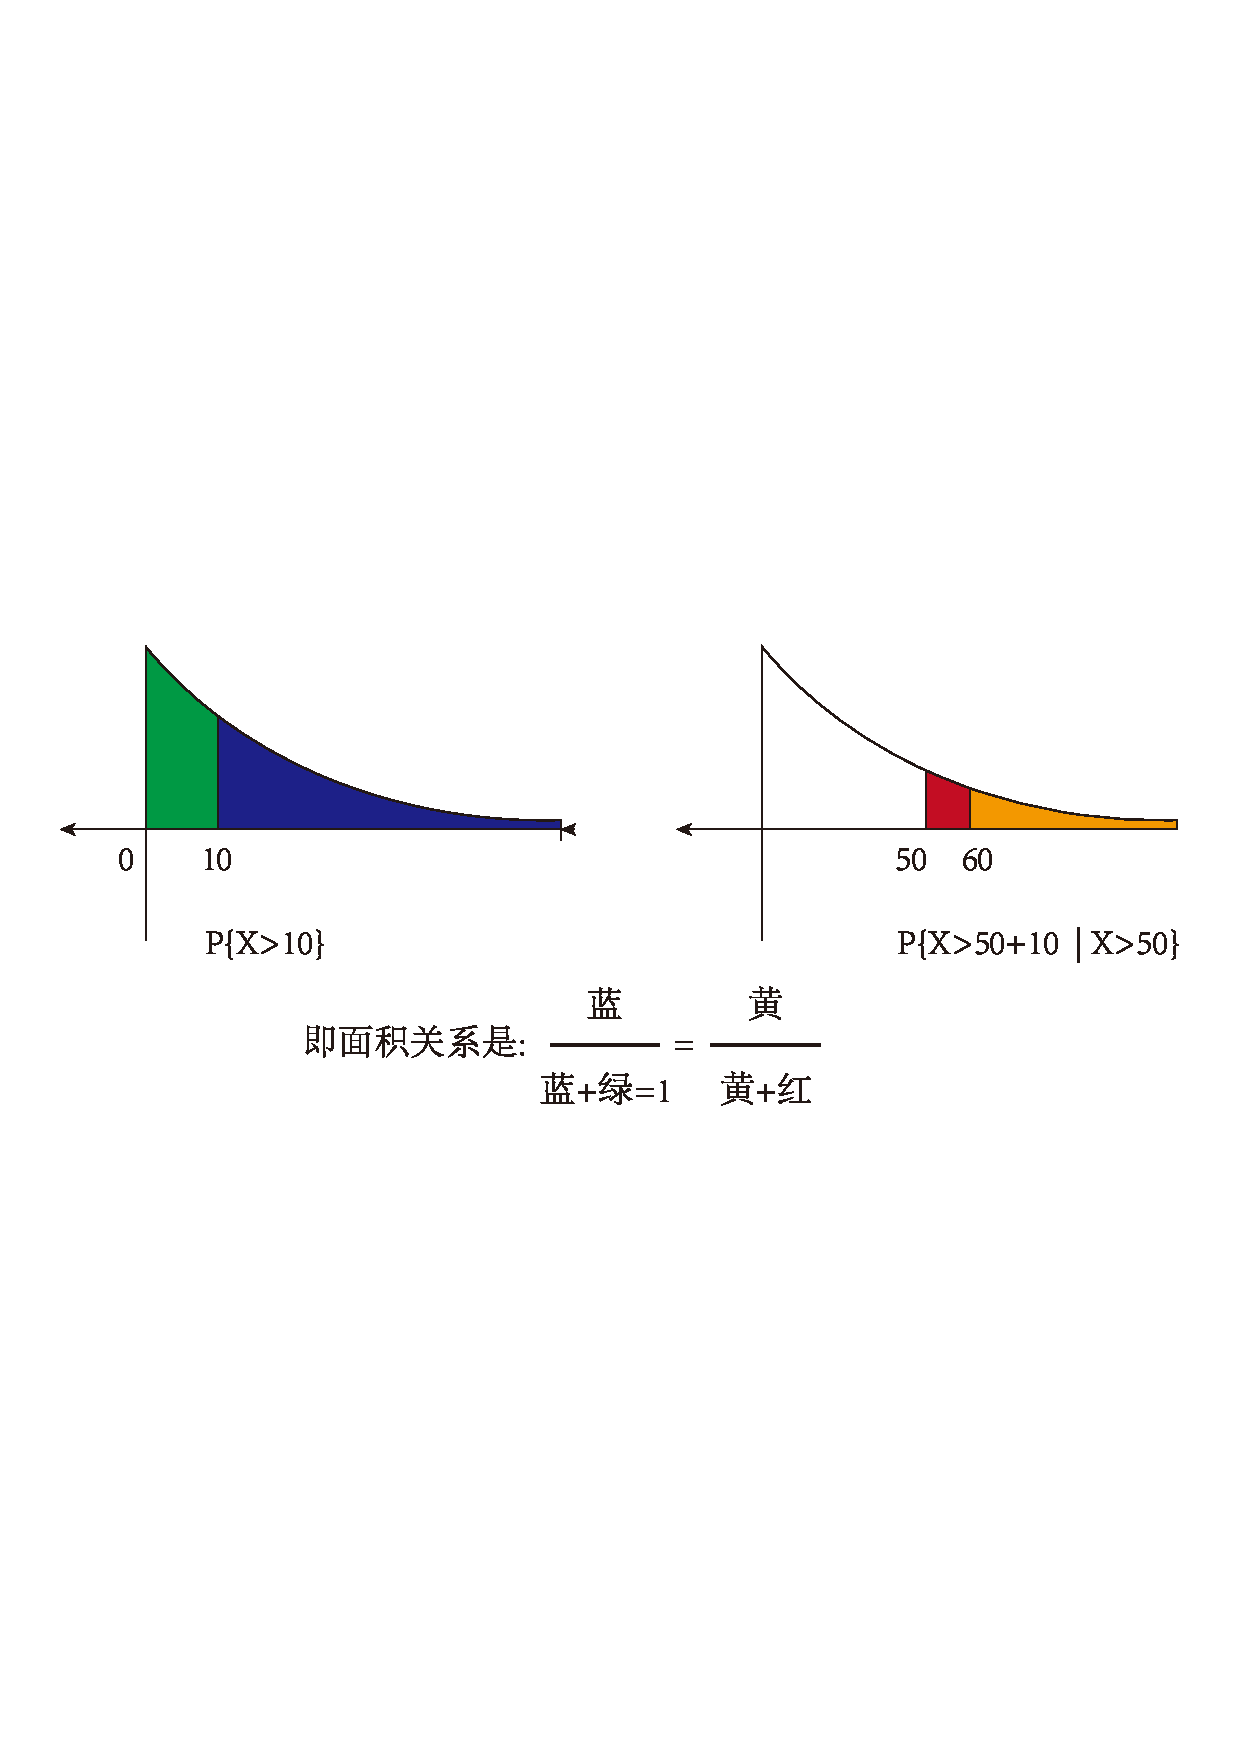
\includegraphics[width=0.7\textwidth]{/0183.pdf}	
	
	
	
	
	
	
	
\section{指数分布的 : 期望$E=\dfrac{1} {\lambda}$,  方差$\sigma^2=(\dfrac{1} {\lambda})^2$}
	
	\begin{tabular}{|l|l|l|}
		\hline
		& 期望E  & 方差$\sigma^2$ \\
		\hline
		泊松分布 Poisson distribution &  $\lambda$ &  $\lambda$ \\
		\hline
		指数分布 Exponential distribution & $ \dfrac{1} {\lambda}$ & $ (\dfrac{1} {\lambda})^2$\\
		\hline
	\end{tabular}
	
	
	
	
	
	
	
	
	
	
	
	
	
	
	
	
	
	
	
\end{document}